% !TEX TS-program = lualatex
%\documentclass[handout]{beamer}
\documentclass{beamer}
\input{../common/misomva}
\newcommand{\misoclasstinytitleslide}{Partially based on material by:  Ulrike von Luxburg, \\[-1em] Gary Miller, Doyle \& Schnell, Daniel Spielman}
\newcommand{\misoclassdate}{}
\usetikzlibrary{graphs}

\begin{document}
% Topic-specific title slide

\newcommand{\topictitle}{Resistive Networks}

\newcommand{\topicsubtitle}{Physics and Effective Resistance}

\MakeTopicSlide

\begin{frame}
\frametitle{Laplacians and Resistive Networks}

\questionbox{How to compute the \textbf{${\rm score} (v,m)$}?}

\begin{block}{Idea$_4$: view edges as conductors}
${\rm score}_4 (v,m) =$ effective resistance between $m$ and $v$
\end{block}
\pause
\begin{columns}[T]
\column{0.5\textwidth}{%
% \vspace{2cm}
\begin{circuitikz}[scale=0.8, transform shape, american, cute inductors, thick]
 \draw
(0,0) to [V, l=\LARGE{$v$}, i^>=\LARGE{$i$}](0,3) to (3,3) to [R, l=\LARGE{$C$}](3,0) to (0,0) 
;\end{circuitikz}
}
\column{0.5\textwidth}{
\begin{align*}
C &\equiv {\rm conductance}\\
R &\equiv {\rm resistance}\\
i &\equiv {\rm current}\\
V &\equiv {\rm voltage}
\end{align*}

}
\bigskip
\pause
\end{columns}
\[
C = \frac{1}{R} \qquad i= CV = \frac{V}{R}
\]
\end{frame}

%%%%%%%%%%%%%%%%%%%%%%%%%%%%%%%%%%%
\begin{frame}
\frametitle{Resistive Networks: Some high-school physics}
\begin{center}
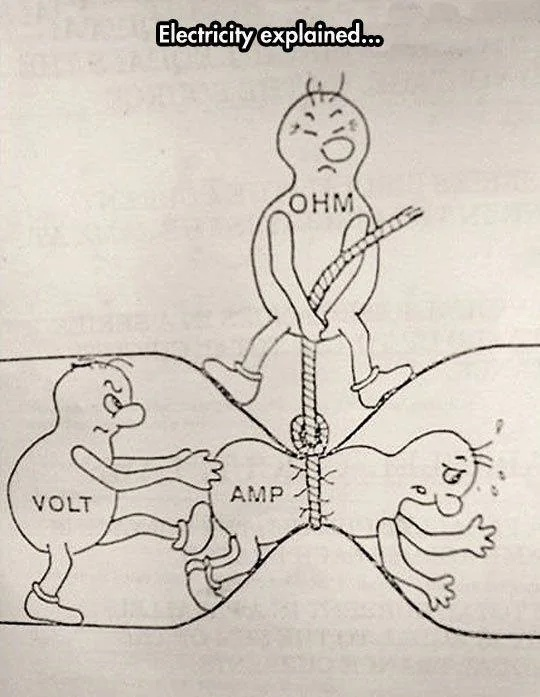
\includegraphics[width=0.5\columnwidth, height=0.65\textheight, keepaspectratio]{../img/ohm_volt_amp}
    
    \medskip
    {\tiny Source: Illustration commonly attributed to Vagonum}
\end{center}
\end{frame}
%%%%%%%%%%%%%%%%%%%%%%%%%%%%%%%%%%%%%%%%%%%%%%%%%%%%%%%%%%%%%
\begin{frame}
\frametitle{Resistive Networks}
\pause
\begin{block}{resistors \gcol{in series}}
\[
R=R_1+\dots+R_n \qquad C = \frac{1}{\frac{1}{C_1}+\dots+\frac{1}{C_\nodes}} \qquad i = \frac{V}{R} 
\]
\end{block}

\pause
\begin{block}{conductors in \gcol{parallel}}
\[
C=C_1+\dots+C_\nodes \qquad i = VC
\]
\end{block}
\pause

\begin{block}{\gcol{Effective Resistance on a graph}}
Take two nodes: $a\ne b$. Let $V_{ab}$ be the voltage between them and $i_{ab}$ the current between them.
Define $R_{ab} = \frac{V_{ab}}{i_{ab}}$ and $C_{ab} = \frac{1}{R_{ab}}.$
\end{block}
\pause
\rightyellbox{We treat the entire graph as a resistor!}
\end{frame}

%%%%%%%%%%%%%%%%%%%%%%%%%%%%%%%%%%%%%%%%%%%%%%%%%%%%%%%%%%%%%

\begin{frame}
\frametitle{Resistive Networks: Optional Homework (ungraded)}

\begin{block}{}
Show that $R_{ab}$ is a metric space.
\end{block}
\pause
\begin{enumerate}
 \item $R_{ab} \geq 0$ \pause
 \item $R_{ab} = 0$ iff $a=b$ \pause
 \item $R_{ab} = R_{ba}$ \pause
 \item $R_{ac} \leq R_{ab} + R_{bc}$ \pause
\end{enumerate}
\rightyellbox {The effective resistance is a distance!}
\end{frame}
%%%%%%%%%%%%%%%%%%%%%%%%%%%%%%%%%%%%%%%%%%%%%%%%%%%%%%%%%%%%%





%%%%%%%%%%%%%%%%%%%%%%%%%%%%%%%%%%%%%%%%%%%%%%%%%%%%%%%

%%%%%%%%%%%%%%%%%%%%







\MakeLastSlide
\end{document}
